
% If you want a large two-column figure (notice '*')
%   Declare this before the start of section for floating arrangement
\begin{figure*}[ht]
    \centering
    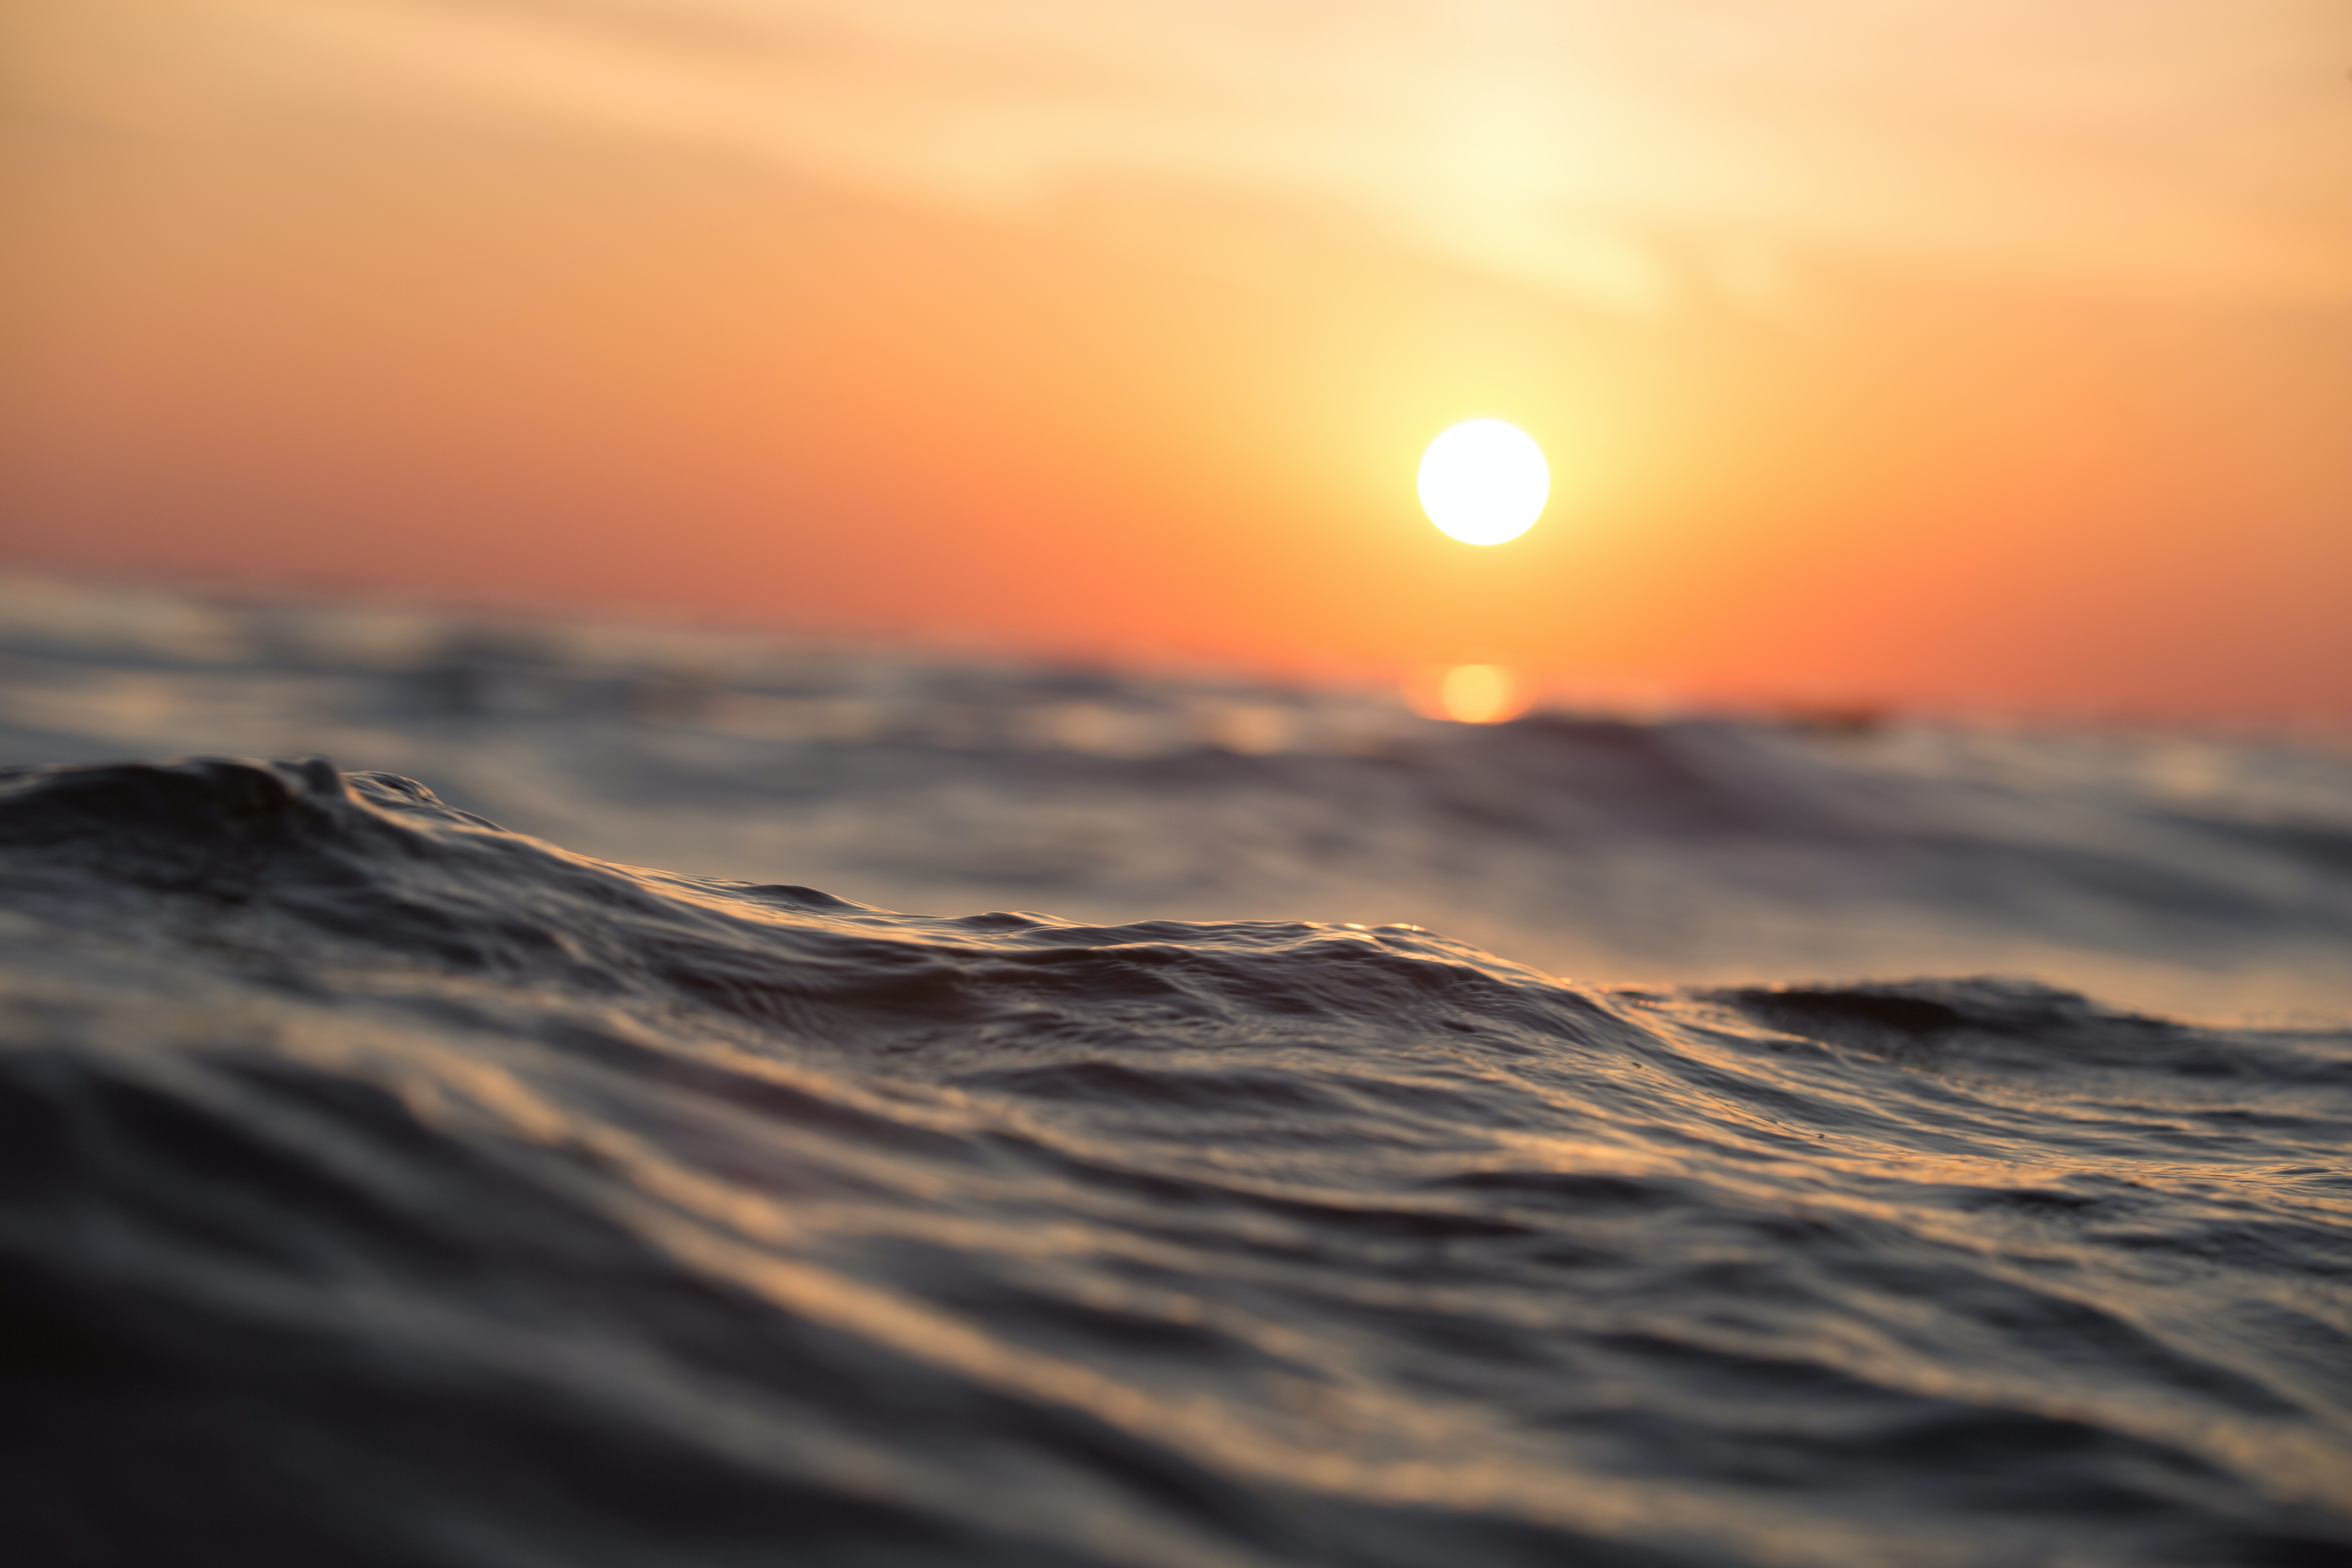
\includegraphics[width=0.95 \linewidth]{sunrise1.jpg}
    \caption{A sunrise}
    \label{fig:sunrise}
    \small
        An inspirational \href{https://www.pexels.com/photo/body-of-water-during-golden-hour-189349/}{Photo by Sebastian Voortman from Pexels} (spanning two columns, at the top of page)
\end{figure*}
% This is how you comment for figures
\am[Regarding 'fig:sunrise']{Maybe add something}


\section{Related Work}

This section has an overview of a technique I use to read papers (I do not want to fill this entire document with \textsc{Ipsum} text). It also has a subsection dedicated to what's included in this work. I am a newbie to the field of literature; please do not take anything seriously. This is just for my personal reference; great if it helps somebody else!

% ---------------------------------------------------

\subsection{Reading Papers}
\label{sub:read-papers}

I essentially have two methods. One is a \emph{time taking deep dive} (TTDD), another is a \emph{staged dive} (SD). If I have to read little literature but gain an in-depth understanding, I use TTDD. If I have to cover a lot of ground but in a shallow manner (like in a literature survey), I use SD.

\subsubsection{TTDD --- Time Taking Deep Dive}

Here, I simply go through each paper (or literature item) one-by-one. Absorbing everything I read and annotating a lot in the paper. This helps me absorb the work as a whole, but I usually end up spending \emph{one full day}. The result is usually that I (usually) understand the work from top-to-bottom and I can start results (in code). At the very least, I have a clear view of the foundations (sometimes the work requires out-of-domain knowledge which I decide on diving into).

\subsubsection{SD --- Staged Dive}

If I have a lot of papers to read and I have to do it quick, I use this method. This is largely inspired from \cite{keshav2007read}. I give three passes to the paper.

\paragraph{Pass 1: Title, abstract, introduction, conclusion}
\label{subsubpara:sd-pass1}

Here, I read the title, abstract, and introduction with great care. I then quickly skim over the images, and the entire paper content (until I reach the conclusion). I then read the conclusion carefully.
After this reading, I decide to continue reading the paper (to gain more information) or to discard it.

\paragraph{Pass 2: Body}
\label{subsubpara:sd-pass2}

If I choose to continue reading, I redo pass 1 (as in \ref{subsubpara:sd-pass1}) and then read the entire paper carefully. Bulk of the annotations come from here. If there are things that I do not understand, I simply highlight them. I also highlight important references here.
After this reading, I decide to continue reading (only if I want to completely duplicate work) or to set it aside.

\paragraph{Pass 3: Full replication}

After finishing \ref{subsubpara:sd-pass1} and \ref{subsubpara:sd-pass2}, if I decide to keep going further, I try and replicate the work.

% ---------------------------------------------------

\subsection{This Document}

Reading the last subsection \ref{sub:read-papers} might have become too boring, so I've put a motivational figure (spanning two columns) in~\autoref{fig:sunrise}. Let's explore some \amswap[New]{content}{concepts}.

You know what, I'll add them as I learn more of \LaTeX.
